   \documentclass[a4paper,14pt]{extarticle}
\usepackage[utf8]{inputenc}
\usepackage[russian]{babel}
\usepackage{graphicx}
\usepackage[top=0.8in, bottom=0.8in, left=0.8in, right=0.8in]
{geometry}
\usepackage{pgfplots}
\usepackage{amsmath}
\usepackage{setspace}
\usepackage{titlesec}
\usepackage{float}
\usepackage{chngcntr}
\usepackage{pgfplots}
\usepackage{amsfonts}
\usepackage{pgfplotstable}
\usepackage{multirow}
\usepackage{karnaugh-map}
\usepackage{tikz,xcolor}
\usepackage{indentfirst} % Красная строка
\usepackage{listings}
\usepackage{amssymb}
\usepackage{xcolor}
\usepackage{hyperref}

\definecolor{linkcolor}{HTML}{0000FF} % цвет ссылок
\definecolor{urlcolor}{HTML}{FF00FF} % цвет гиперссылок

\hypersetup{pdfstartview=FitH, linkcolor=linkcolor,urlcolor=urlcolor, colorlinks=true}


\titleformat{\section}[hang]
  {\bfseries}
  {}
  {0em}
  {\hspace{-0.4pt}\large \thesection\hspace{0.6em}}
  
  
\titleformat{\subsection}[hang]
  {\bfseries}
  {}
  {0em}
  {\hspace{-0.4pt}\large \thesubsection\hspace{0.6em}}

%\linespread{1.3} % полуторный интервал
%\renewcommand{\rmdefault}{ftm} % Times New Roman

\newcommand{\nx}{\overline{x}}
\newcommand{\p}{0.31}
\newcommand{\scale}{1.4}

\counterwithin{figure}{section}
\counterwithin{equation}{section}
\counterwithin{table}{section}

\begin{document}
\begin{titlepage}
\centering
Санкт-Петербургский политехнический университет Петра Великого \\
\vspace{0.15cm}
Кафедра компьютерных систем и программных технологий \\
\vspace{6.5cm}

{\centering \textbf{Отчёт по лабораторной работе} \\ 
\vspace{0.15cm}
\textbf{Дисциплина}: Телекоммуникационные технологии \\
\vspace{0.15cm}
\textbf{Тема}: Линейная фильтрация} \\


\vspace{6.5cm}

\begin{table}[H]
\begin{tabular}{p{\textwidth}@{}r}
{Выполнил студент гр. 33501/2} \hfill {Вахаев И.Н.} \\
{Преподаватель} \hfill {Богач Н.В.} \\
\end{tabular}
\end{table}
\vfill

{\centering Санкт-Петербург \\ 
\vspace{0.15cm}
\today}
\end{titlepage}

\tableofcontents
\newpage

\section{Цель работы}

Изучить воздействие ФНЧ на тестовый сигнал с шумом.

\section{Постановка задачи}

Сгенерировать гармонический сигнал с шумом и синтезировать ФНЧ. Получить сигнал во временной и частотной областях до и после фильтрации. Сделать выводы о воздействии ФНЧ на спектр сигнала.

\section{Теоретический раздел}

\subsection{Общие сведения о линейной фильтрации}

Линейный фильтр — динамическая система, применяющая некий линейный оператор ко входному сигналу для выделения или подавления определённых частот сигнала и других функций по обработке входного сигнала. Линейные фильтры широко применяются в электронике, цифровой обработке сигналов и изображений, в оптике, теории управления и других областях.

Линейную фильтрацию широко используют в системах передачи информации для обработки сигналов. Объясняется это прежде всего простотой реализации линейных фильтров, которые легко синтезируются и существованием развитой теории их построения. Они являются неотъемлемой частью любого приемного устройства. С их помощью осуществляется как додетекторная, так и последетекторная обработки сигналов. С помощью лишенных фильтров сигналы разделяются в многоканальных системах передачи.

Линейная фильтрация сигнала для выделения его из смеси сигнал шум является одним из основных процессов, осуществляемых в любом радиоприемном устройстве. В основе фильтрации лежит использование частотной избирательности колебательных цепей. На протяжении первых 50 - 60 лет развития радиотехники к подобным частотным фильтрам предъявлялось требование возможно более равномерного проп екания спектра сигнала и возможно более полного подавления частот вне этого спектра. Идеальным считался фильтр с прямоугольной П - образной АЧХ.


\section{Ход работы}

\subsection{Генерация гармонического сигнала с шумом}

Была разработана схема, в которой к синусоидальному сигналу добавляется белый шум. Схема продемонстрирована на рисунке \ref{001}.

\begin{figure}[H]
\center{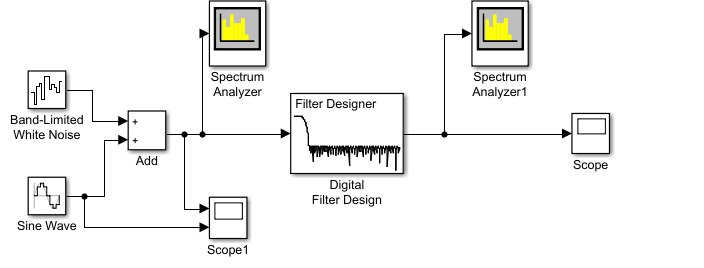
\includegraphics[width=1\linewidth]{screen/1.png}}
\caption{Схема разработанная в Simulink.}
\label{001}
\end{figure}

При сложении синусоидального сигнала(Sine Wave) и белого шума(Band-Limited White Noise) получили зашумленный сигнал, представленный на рисунке \ref{002}.

\begin{figure}[H]
\center{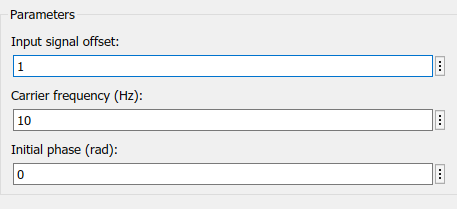
\includegraphics[width=1\linewidth]{screen/2.png}}
\caption{Зашумленный сигнал.}
\label{002}
\end{figure}

Также был получен спектр зашумленного сигнала (Рисунок \ref{003}).

\begin{figure}[H]
\center{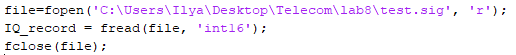
\includegraphics[width=1\linewidth]{screen/3.png}}
\caption{Спектр зашумлённого сигнала.}
\label{003}
\end{figure}


\subsection{Фильтрация сигнала с шумом}

Была проведена фильтрация сигнала с шумом с использованием фильтра Kaiser 65 порядка. Фильтр представлен на рисунке \ref{004}. 

\begin{figure}[H]
\center{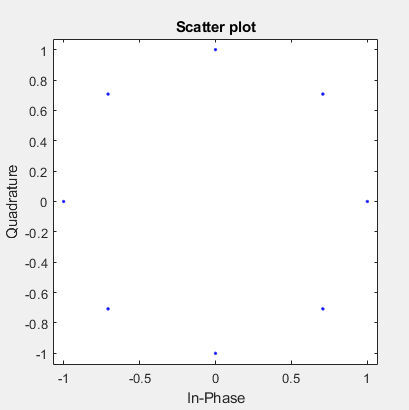
\includegraphics[width=1\linewidth]{screen/4.png}}
\caption{Фильтр Kaiser 65 порядка.}
\label{004}
\end{figure}

Получили отфильтрованный сигнал (Риснок \ref{005}) и спектр отфильтрованного сигнала (Рисунок\ref{006}).

\begin{figure}[H]
\center{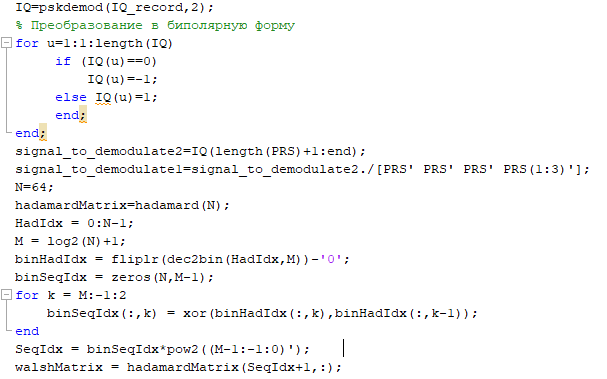
\includegraphics[width=1\linewidth]{screen/5.png}}
\caption{Исходный и отфильтрованный сигнал.}
\label{005}
\end{figure}

\begin{figure}[H]
\center{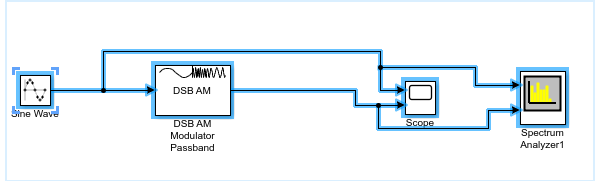
\includegraphics[width=1\linewidth]{screen/6.png}}
\caption{Спектр отфильтрованного сигнала.}
\label{006}
\end{figure}

Фильтр с 65 порядком довольно плохо отфильтровал зашумлённый сигнал. Для лучшего результата порядок фильтра был увеличен до 129 (Рисунок\ref{007}).

\begin{figure}[H]
\center{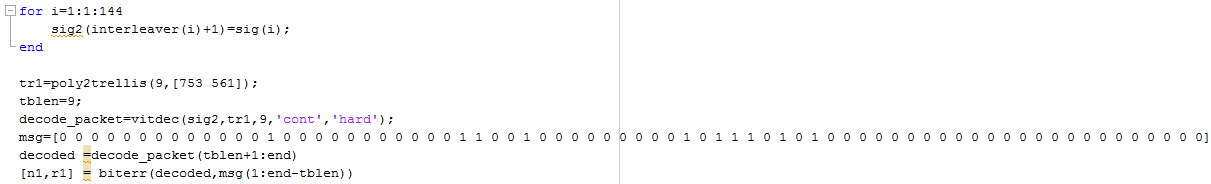
\includegraphics[width=1\linewidth]{screen/7.png}}
\caption{Фильтр 129 порядка.}
\label{007}
\end{figure}

Получили следующий вид отфильтрованного сигнала (Рисунок\ref{008}).

\begin{figure}[H]
\center{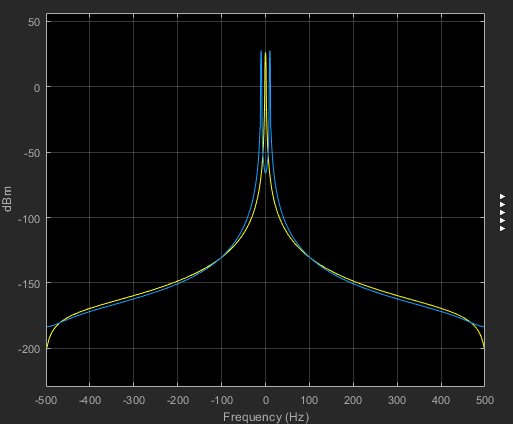
\includegraphics[width=1\linewidth]{screen/8.png}}
\caption{Исходный и отфильтрованный сигнал.}
\label{008}
\end{figure}

Также получили его спектр (Рисунок\ref{009}).

\begin{figure}[H]
\center{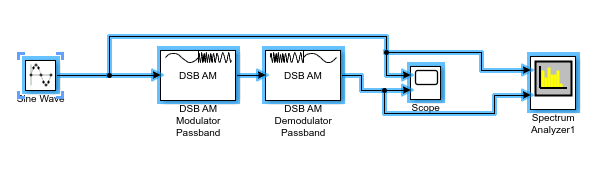
\includegraphics[width=1\linewidth]{screen/9.png}}
\caption{Спектр отфильтрованного сигнала.}
\label{009}
\end{figure}

Порядок фильтра был увеличен на ещё большее значение - 206.

В результате получили данный отфильтрованный сигнал (Рисунок\ref{010}).

\begin{figure}[H]
\center{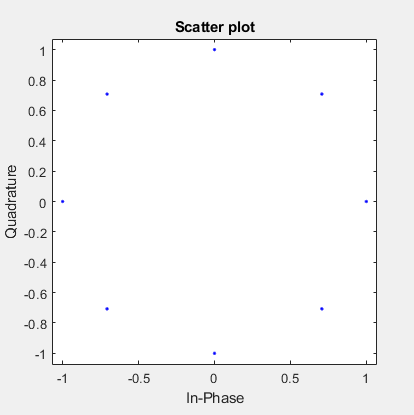
\includegraphics[width=1\linewidth]{screen/10.png}}
\caption{Исходный и отфильтрованный сигнал.}
\label{010}
\end{figure}

Спектр (Рисунок\ref{011}) отфильтрованного сигнала принял следующий вид:

\begin{figure}[H]
\center{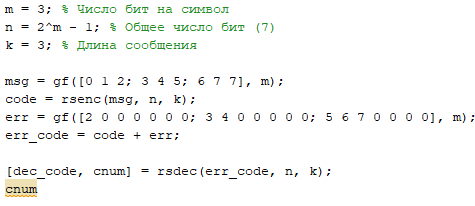
\includegraphics[width=1\linewidth]{screen/11.png}}
\caption{Спектр отфильтрованного сигнала.}
\label{011}
\end{figure}

Видно, что с повышением порядка данного фильтра сигнал лучше фильтруется, однако чем выше порядок, тем выше задержка фильтрации.

По полученным результатам можно сделать вывод, что фильтр работает достаточно хорошо, так как отфильтрованный зашумленный сигнал почти соответствует исходному.


\section{Выводы}

В ходе работы был исследован фильтр из примера библиотеки Simulink, а также создана схема для генерации синусоидального сигнала, его зашумления и фильтрации.
При сравнении исходного и отфильтрованного сигналов, а также их спектров видно, что фильтр работает правильно. Фильтрация помогла избавиться от значительной части шума, пусть и не всей, так как белый шум распределён по всем частотам и он существует на тех, что и исходный сигнал, который его искажает.




\end{document}